\section{Results}
For country-product bi-partite networks,  Caldarelli et al. \cite{caldarelli2012network} found that the ranking of countries correlates reasonably well with their ranking in terms of GDP, with Spearman correlation $\approx 0.4$ for calibration values $\alpha \approx 1.1$ and $\beta \approx 0.8$. Similarly, we studied the correlations of the article-editor ranking model with grand-truth exogenous values. We studied how these correlations evolve as more edits are contributed to a category of Wikipedia articles. Finally, we investigated the values of calibrated $\alpha$ and $\beta$ in the context of Wikipedia open collaboration.

Figure \ref{fig:rhotime} shows the evolution of the maximum achievable rank correlation, Spearman $\rho$, between $\mathbf{w}^*_a$ versus $\mathbf{v}_a$ and $\mathbf{w}^*_e$ versus $\mathbf{v}_e$, respectively, as a function of time for each of the twelve categories.  The maximum rank correlation is obtained by a grid search. In our visualizations we draw a contour around the areas in the top 95\textsuperscript{th} percentile.
The correlations are generally quite high ( $ 0.46 < \rho_e < 0.75$ with $\langle \rho_e\rangle = 0.64$ for editors and $0.57 < \rho_a < 0.91$ with $\langle \rho_a\rangle = 0.72$ ). Yet the rank correlations of editors remain overall smaller than rank correlations obtained for articles. This difference might be due to the roughness of the grand truth for editors $v_e$, expressed in labor-hours, compared to the quality of $v_a$, which is an aggregate measure of five precise quality metrics. Nevertheless, the correlation of editors' ranking with $v_e$ increases: $\rho_e$ exhibits a convex increase over time, suggesting that it takes time (i.e., lots of edits) to capture well the expertise of editors as well as for editors. 


\begin{figure}[!t]
\centering
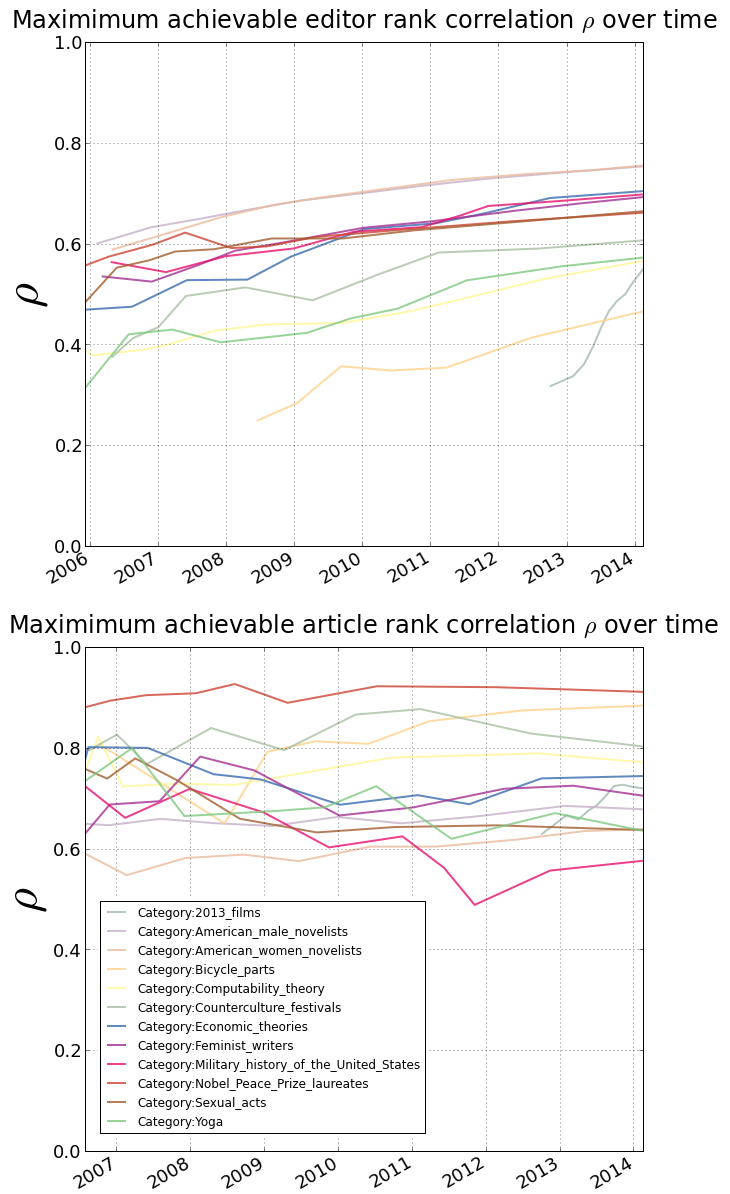
\includegraphics[width=0.9\columnwidth]{Figures/rho_combined.png}.
\caption{Evolution of Spearman $\rho$ rank correlations between the ranking obtained from the calibrated model and the grand-truth values for each category and for editors (upper panel)  and articles (lower panel). The correlations are generally quite high : $ 0.46 < \rho_e < 0.75$ with $\langle \rho_e\rangle = 0.64$ for editors and $0.57 < \rho_a < 0.91$ with $\langle \rho_a\rangle = 0.72$. $\rho_{a}$  is stable over time, which means that the quality of articles can be well captured early on by the model. However, $\rho_e$ exhibits a convex increase over time, suggesting that it takes time (i.e., lots of edits) to capture well the expertise of editors.}
\label{fig:rhotime}
\end{figure}



We now turn finding the values of $\alpha$ and $\beta$ for which best correlation is achieved.  

With regards to \eqref{eqsim}, we can see the similarity of $w^*$ is related to the product of two expressions. Consider the limit as either $\alpha$ or $\beta$ approach $0$ independently., If one expression becomes unity, then the other expression dominates. In the article plot of Figure \ref{fig:landscape} our solution spaces moves linearly from $ \beta < 1 , \alpha \approx 0$ meaning that successful articles are largely uninfluenced by quality of the work its editors do elsewhere. This "spine" at $alpha = 0$ is a common feature in all our categories.
For editors, on the other hand there are more complex solution spaces. In  \ref{fig:landscape}, we find a maximizing area roughly bounded $ -2  <\alpha < 1 , 0 < \beta > 2 $. This means that fit editors are characterized by a the spectrum defined by the extremes (i) minorly by the quality of the articles they've contributed to and partly by the size of their touched articles portfolio, or (ii) in the case that $\alpha < 0$ that contributed-to article quality is supremely important and that touching many articles is anti-important.

The question remains if the intersection of the solution spaces for $\rho_a$ and $\rho_e$ is nonempty. That is whether the we can find values of $\alpha$ and $\beta$ for which our editor ranking and article ranking are simultaneously optimized. We exploit two empirical facts from our data: the clear solution for article rankings that $alpha = 0$, and that for editor rankings the 95\textsuperscript{th} percentile maximizing boundary always includes values at $\alpha = 0$. Therefore, with $\alpha = 0$, we solve for $\beta$ in the editor ranking that maximizes $\rho_e$ - and thus $\rho_a$ simultaneously. 

In \ref{landscape} the simultaneous maximizing solution exists at $\alpha = 0, \beta \approx 0.7$. This means that article ubiquity is more important than prolific editor output in ranking editors and articles.

\ref{tab:maxbeta} lists each category by its maximizing $\beta$ value. Recall higher $\beta$ indicates more importance of article ubiquity. Noting that \eqref{eqsim} has a singularity at $\beta = 1$, we see that if $\beta > 1$ we actually enter into the symmetric reflection of the plot where the sign of our correlations is reverse. Since the magnitude of the anti-correlation is equal along the $\alpha = 0$ spine, this is not a problem as the predictive power remains just as high.
We also find, as in the first two entries of \ref{tab:maxbeta}, that a maximizing $\beta$ may be $0$, in this case, the original \ref{HHalgo} algorithm would be just as predictive. 

\begin{table}
\end{table}
\begin{tabular}{lll}
\toprule
                                       Category &   Spearman $\rho$ &  $\beta$ \\
\midrule
                         Bicycle parts &  0.8953 &     0 \\
 Military history of the US &  0.5767 &     0 \\
                  Computability theory &  0.7748 &  0.32 \\
               American male novelists &  0.6729 &   0.4 \\
                            2013 films &  0.7220 &  0.48 \\
                     Economic theories &  0.7382 &  0.48 \\
              American women novelists &  0.6304 &  0.64 \\
                      Feminist writers &  0.7036 &  0.72 \\
                                  Yoga &  0.6355 &  1.12 \\
           Nobel Peace Prize laureates &  0.9096 &   1.2 \\
              Counterculture festivals &  0.8031 &  1.36 \\
                           Sexual acts &  0.6341 &  1.52 \\
\bottomrule
\end{tabular}
\caption{Maximizing values of $\beta$ when $\alpha = 0$, sorted by $\beta$.}
\label{tab:maxbeta}
\end{table}

\begin{figure}[!t]
\centering
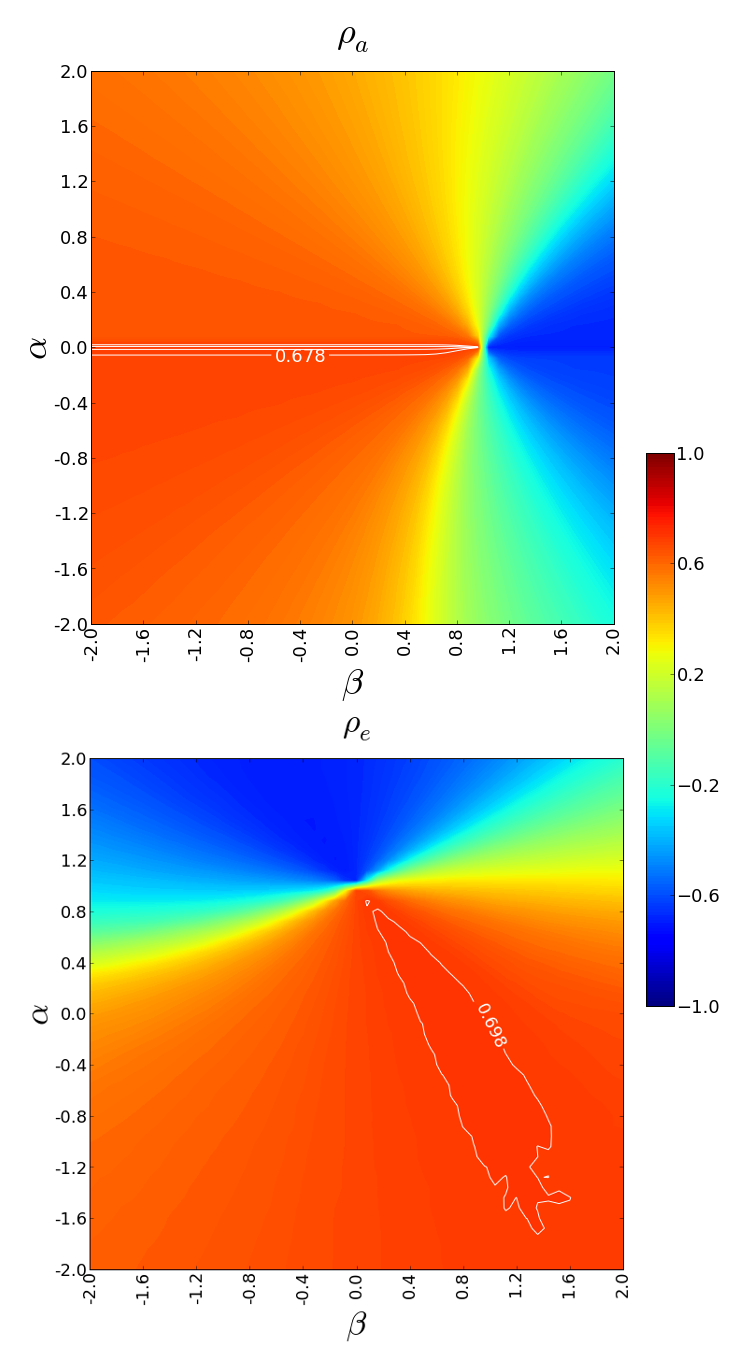
\includegraphics[width=0.9\columnwidth]{Figures/contour_fem_combined.png}.
\caption{Typical landscape of maximum correlation as a function of $\alpha$ and $\beta$ for articles (upper panel) and editors (lower panel). The contour line shows the 95\textsuperscript{th} percentile of the rank correlation over the landscape.}
\label{fig:landscape}
\end{figure}

%\clearpage


%\subsection{Article-Editor Ranking Calibration}
%
%Having our endogenous and exogenous variables now, we perform tests to
%$\underset{\alpha, \beta}{\operatorname{argmax}} \rho(\alpha, \beta)$, the pair that maximizes our spearman rank correlation between  $\mathbf{w^{*}_{e}}$ and $v_e$. We also do so for $\mathbf{w^{*}_{a}}$ and $v_a$.
%
%First we used a general purpose maximizing algorithm to find maximizing values. Secondly we performed a grid search with visual inspection. Overall we find smooth landscapes. The two methods verified each other's results. \ref{fig:contour_fem} shows the correlation landscape for Category:Feminist Writers calibrating both articles and editors.
%
%The results of calibrating our model are encouraging as we find high correlations between the results of our $w^*_e$ algorithm and our exogenous variables $v$. 
%
%We define $\rho$ at the maximum achievable spearman rank correlation between $w^*$ and $v$ for editors or articles, by category, and over time. The variation of $\rho$, by for editor for any category ranges from 0.75 to 0.46 with a mean 0.64.  That same statistic for articles is articles from 0.91 to 0.57 with a mean of 0.72, which is overall higher.
%
% 
%From snapshotting we see view $\rho$ as  a function of time. In the case of editors we see increasing trends in all categories over time in an asymptotic way. This means that $w^*_e$ benefits from incorporating more contribution history. That is, as a category matures we can better predict successful editors from which articles they edit. As for being able to predict article quality, from the start of a category's history the correlations remain high and  stable. It is easier to predict an articles quality based on who has edited it.  \ref{fig:rhotime}
%
%\begin{figure}[!t]
%\centering
%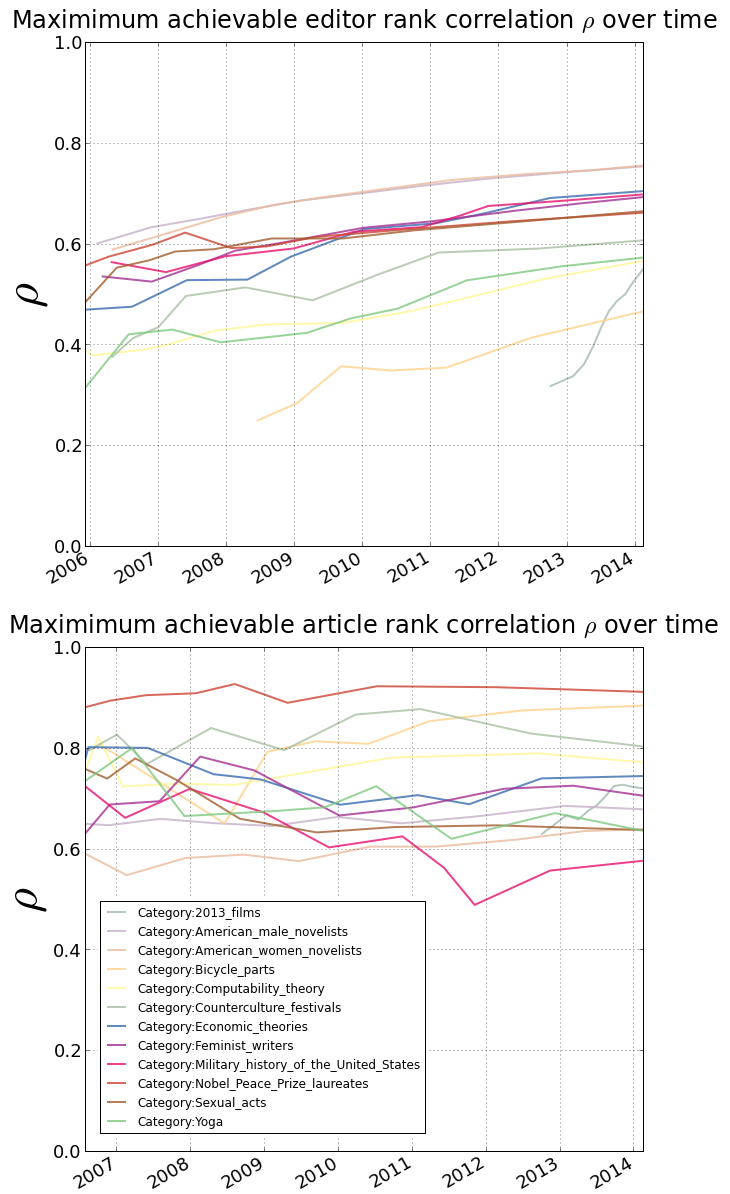
\includegraphics[width=0.9\columnwidth]{Figures/rho_combined.png}.
%\caption{$\rho$ over time, by category and type}
%\label{fig:rhotime}
%\end{figure}
%
%
%\subsection{Negative values of $\alpha$ and $\beta$}
%Another surprising result is that we find at times, negative values for $\alpha$ and $\beta$.
%
%To understand the results, we must have a firm grasp on what $\alpha$ and $\beta$ mean. They are more easily understood by roughly rewriting $\mathbf{w^*}$ as:
%\begin{equation}
%\begin{cases}
%w^{*}_{e} \sim k^{1-\beta}_{e} \langle k_{a}^{-\alpha}\rangle_e \\
%w^{*}_{a} \sim k^{1-\alpha}_{a} \langle k_{e}^{-\beta}\rangle_a
%\end{cases} \label{eqsim}
%\end{equation}
%
%Our solution spaces are not single point but a 2-dimensional area, similar to what found in \cite{caldarelli2012network}. A reason for this is the fact that we are using the spearman ranking correlation, once a ranking is achieved, $\alpha$ and $\beta$ can perturb without adjusting the ranking. 
%
%In these areas we see trends in there being important axes shown by the maximizing segments, which represent a several explanations for the article behaviour behaviour.
%
%With regards to \eqref{eqsim}, we can see the similarity of $w^*$ is related to the product of two expression. Values of $\alpha$ and $\beta$ can make the one of the product approach one or and so the other parameter may dominate. In the article plot of \ref{fig:contour_fem} our solution spaces moves linearly from $0 <\alpha <1 , \beta \approx 0$ meaning that successful editors are charcterized, by an equal balance of their edit count, and the average article quality of articles they've edited. At the other end $\alpha < - 1 , \beta > 1$ anti-importance of their how man articles they've edited, but high importance on the quality of edits.
%
%This seems quite natural to say, but $\alpha$ and $\beta$ need not vary together at all, and could be in different quadrants of the landscape each describing a different success strategy.
%
%\begin{figure}[!t]
%\centering
%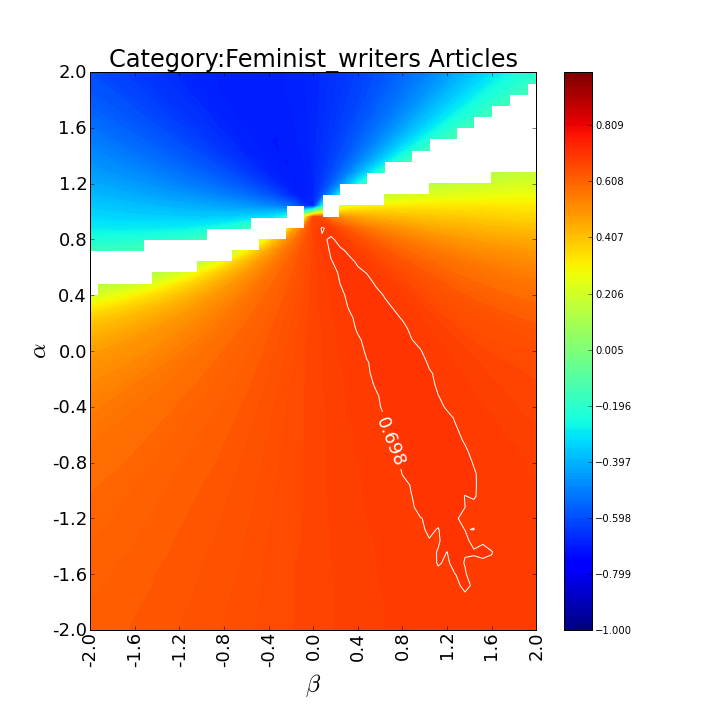
\includegraphics[width=0.9\columnwidth]{Figures/contour_fem.png}.
%\caption{Heatmaps of Spearman Rank Correlation between endogenous and exogenous ranks, 95$^{th}$ percentile  of correlations circled
%Upper panel: articles - $w^*_a ~ v_a$
%Lower panel editors - $w^*_e ~ v_e$
%White indicates that correlation was not significant $p<0.05$ } 
%\label{fig:contour_fem}
%\end{figure}
%
%\subsection{$\rho$ increases over time.}

	



